\documentclass[10pt,a4paper]{article}
\usepackage[margin=1.9cm,top=1.6cm,bottom=1.7cm]{geometry}
\usepackage{amsmath,amssymb,graphicx,booktabs,array,microtype,caption,enumitem,float,hyperref}
\usepackage[T1]{fontenc}\usepackage{lmodern}
\captionsetup{font=small,labelfont=bf,skip=3pt}
\setlength{\parskip}{2pt}\setlength{\parindent}{0pt}
\setlist{nosep,leftmargin=1.2em}
\renewcommand{\arraystretch}{1.08}
\newcommand{\RT}{R T}
\hypersetup{hidelinks}
\makeatletter\renewcommand\section{\@startsection{section}{1}{0pt}{6pt}{2pt}{\normalfont\large\bfseries}}\makeatother

\begin{document}
\begin{center}
{\Large\bfseries Thermodynamic Properties of Real Gases from Cubic Equations of State}\\[2pt]
{\large PVT behaviour, residual enthalpy and entropy, and pure-component fugacity}\\[3pt]
Ayush Vishwakarma (2025CH71662) \quad Naman Garg (2025CH71053)\\[1pt]Tutorial group: 2 \quad Submitted: 10 November 2026
\end{center}
\vspace{-4pt}\hrule\vspace{3pt}

\section{Scope}
The program \texttt{cubic\_eos.py} (Python 3, NumPy/SciPy) covers the three stages of the project for a pure gas: (i) PVT behaviour from four cubic equations of state (EOS) -- van der Waals (vdW), Redlich--Kwong (RK), Soave--Redlich--Kwong (SRK) and Peng--Robinson (PR); (ii) the thermodynamic properties $H$ and $S$ (residual and total); (iii) the pure-component fugacity $f$ and fugacity coefficient $\phi$, including the vapour pressure from equal fugacity. A database of 22 gases ($T_c$, $P_c$, $\omega$, ideal-gas $C_p$) is included and any other gas can be entered by hand.

\section{Theory}
\textbf{Generic cubic EOS.} All four models are special cases of
\begin{equation}
P=\frac{RT}{V-b}-\frac{a(T)}{(V+\epsilon b)(V+\sigma b)},\qquad b=\Omega\frac{RT_c}{P_c},\quad a(T)=\Psi\,\alpha(T_r)\frac{R^2T_c^2}{P_c},
\end{equation}
with the constants of Table~\ref{tab:eos} ($\kappa_{SRK}=0.480+1.574\omega-0.176\omega^2$, $\kappa_{PR}=0.37464+1.54226\omega-0.26992\omega^2$, $\alpha=[1+\kappa(1-\sqrt{T_r})]^2$).
\begin{table}[h]\centering\small
\begin{tabular}{lccccc}\toprule
EOS & $\sigma$ & $\epsilon$ & $\Omega$ & $\Psi$ & $\alpha(T_r)$ \\\midrule
vdW & 0 & 0 & 1/8 & 27/64 & 1\\
RK & 1 & 0 & 0.08664 & 0.42748 & $T_r^{-1/2}$\\
SRK & 1 & 0 & 0.08664 & 0.42748 & $[1+\kappa_{SRK}(1-\sqrt{T_r})]^2$\\
PR & $1+\sqrt2$ & $1-\sqrt2$ & 0.07779 & 0.45724 & $[1+\kappa_{PR}(1-\sqrt{T_r})]^2$\\\bottomrule
\end{tabular}\caption{Constants of the generic cubic EOS (the program uses the unrounded values).}\label{tab:eos}
\end{table}

\textbf{PVT.} With $A=aP/(RT)^2=\Psi\alpha P_r/T_r^2$ and $B=bP/RT=\Omega P_r/T_r$, Eq.~(1) becomes the cubic in $Z=PV/RT$
\begin{equation}
Z^3+\big[(\epsilon+\sigma)B-(1+B)\big]Z^2+\big[\epsilon\sigma B^2-(1+B)(\epsilon+\sigma)B+A\big]Z-\big[(1+B)\epsilon\sigma B^2+AB\big]=0 .
\end{equation}
Three real roots occur below $T_c$ in a pressure window (the van der Waals loop); the smallest is liquid-like, the largest vapour-like, the middle one is mechanically unstable. For $(T,V)$ input, $P$ is evaluated directly from Eq.~(1).

\textbf{Fugacity.} With $q=A/B$ and $I=\frac{1}{\sigma-\epsilon}\ln\frac{Z+\sigma B}{Z+\epsilon B}$ ($I=B/Z$ for vdW),
\begin{equation}
\ln\phi=Z-1-\ln(Z-B)-qI,\qquad f=\phi P .
\end{equation}
When three roots exist the stable phase is the one with the lowest $\ln\phi$ (lowest Gibbs energy). The vapour pressure $P^{sat}(T)$ is the pressure at which $\ln\phi^L=\ln\phi^V$.

\textbf{Enthalpy and entropy.} The residual (departure) functions follow from $H^R/RT=-T(\partial\ln\phi/\partial T)_P$ and $S^R/R=H^R/RT-\ln\phi$; with $d\!\ln\alpha/d\!\ln T_r$ (0, $-\tfrac12$, $-\kappa\sqrt{T_r}/\sqrt\alpha$ for vdW, RK, SRK/PR):
\begin{equation}
\frac{H^R}{RT}=Z-1+\Big(\frac{d\ln\alpha}{d\ln T_r}-1\Big)qI,\qquad
\frac{S^R}{R}=\ln(Z-B)+\frac{d\ln\alpha}{d\ln T_r}\,qI,\qquad G^R=RT\ln\phi=H^R-TS^R .
\end{equation}
The total properties add the ideal-gas part, with $C_p^{ig}/R=A_0+B_0T+C_0T^2+D_0T^{-2}$ and reference $T_0=298.15$ K, $P_0=1$ bar ($H^{ig}=S^{ig}=0$):
\begin{equation}
H=\int_{T_0}^{T}C_p^{ig}dT+H^R,\qquad S=\int_{T_0}^{T}\frac{C_p^{ig}}{T}dT-R\ln\frac{P}{P_0}+S^R .
\end{equation}
Property \emph{changes} between two states, $\Delta H=H_2-H_1$ and $\Delta S=S_2-S_1$, are independent of the reference state; the program calculates them for any pair $(T_1,P_1)\to(T_2,P_2)$, including across a phase change.

\section{Program structure and algorithm}
\begin{enumerate}
\item \textbf{Input (prompted):} gas (name/formula or custom $T_c,P_c,\omega$, $C_p$ coefficients), EOS, and $(T,P)$ or $(T,V)$; units such as \texttt{25C}, \texttt{5MPa}, \texttt{1atm}, \texttt{700psi} are accepted.
\item \textbf{Roots:} the cubic (2) is solved with \texttt{numpy.roots}; each root is polished by Newton iteration (important for the tiny liquid root at low $P$) and roots with $Z\le B$ ($V\le b$) are rejected.
\item \textbf{Phase and properties:} for every root $Z,\ \ln\phi,\ H^R,\ S^R,\ H,\ S$ are evaluated by Eqs.~(3)--(5). The root with minimum $\ln\phi$ is the stable phase; the label (vapour, liquid, supercritical fluid, saturated) is obtained by comparison with $P^{sat}(T)$ and $T_c$.
\item \textbf{Saturation:} the two extrema of the isotherm are located from $\partial P/\partial V=0$ (a quartic in $V$); they bracket $P^{sat}$, which is found by Brent's method on $g(\ln P)=\ln\phi^L-\ln\phi^V$ (it returns $\Delta H^{vap}=H^V-H^L$ and $\Delta S^{vap}=\Delta H^{vap}/T$).
\item \textbf{Interface:} running \texttt{python cubic\_eos.py} starts a guided dialogue that prompts for everything needed (gas, EOS, type of calculation, $T$, $P$ or $V$) and repeats until the user quits. Menu: state at $(T,P)$; state at $(T,V)$; vapour pressure, saturated fugacity and $\Delta H^{vap}$; table versus $P$ with optional CSV export; $\Delta H,\Delta S$ between two states; comparison of all four EOS.
\end{enumerate}
Robustness: the solver was run for all 22 gases $\times$ 4 EOS at $T_r=0.45,0.5,0.6,0.8,0.95,0.99,0.999$ (644 cases) without failure.

\section{Verification}
\texttt{validate.py} runs the following automatic tests (all pass).
\begin{table}[h]\centering\small
\begin{tabular}{p{7.2cm}p{8.6cm}}\toprule
Test & Result\\\midrule
Ideal-gas limit ($P\to0$) for all gases/EOS & $Z,\phi\to1$, $H^R,S^R\to0$\\
$H^R=-RT^2(\partial\ln\phi/\partial T)_P$ and $S^R$ identity, 828 states (central differences) & max.\ error $9\times10^{-8}$ in $H^R/RT$ and $S^R/R$\\
Equal fugacity at $P^{sat}$ (112 cases) & $|\ln\phi^L-\ln\phi^V|<10^{-14}$\\
Clapeyron: $\Delta H^{vap}$ from $H^R$ vs.\ $T\Delta V\,dP^{sat}/dT$ & relative difference $\le1.5\times10^{-7}$\\
Closed-form $\int C_p\,dT$, $\int C_p/T\,dT$ vs.\ numerical quadrature & $3\times10^{-16}$\\
Independent code (CoolProp PR and SRK backends, 58 states) & $Z$, $\ln\phi$, $H^R$, $S^R$ agree to $<10^{-8}$\\
\bottomrule
\end{tabular}\caption{Verification tests. The last row confirms Eqs.~(2)--(4) are implemented exactly as in an independent code.}
\end{table}

\section{Results}
\textbf{PVT and phase behaviour.} Fig.~\ref{fig:1}a shows PR isotherms of n-butane with the van der Waals loop below $T_c$ and the saturation dome from the fugacity calculation; the critical isotherm has the inflection at $P_c$. Fig.~\ref{fig:1}b compares $Z(P)$ of CO$_2$ at 350 K ($T_r=1.15$) with the CoolProp reference Helmholtz EOS: all models are exact in the limit $P\to0$; vdW is poor, PR and RK follow the reference, SRK over-predicts $Z$ around 150--250 bar.

\begin{figure}[h]\centering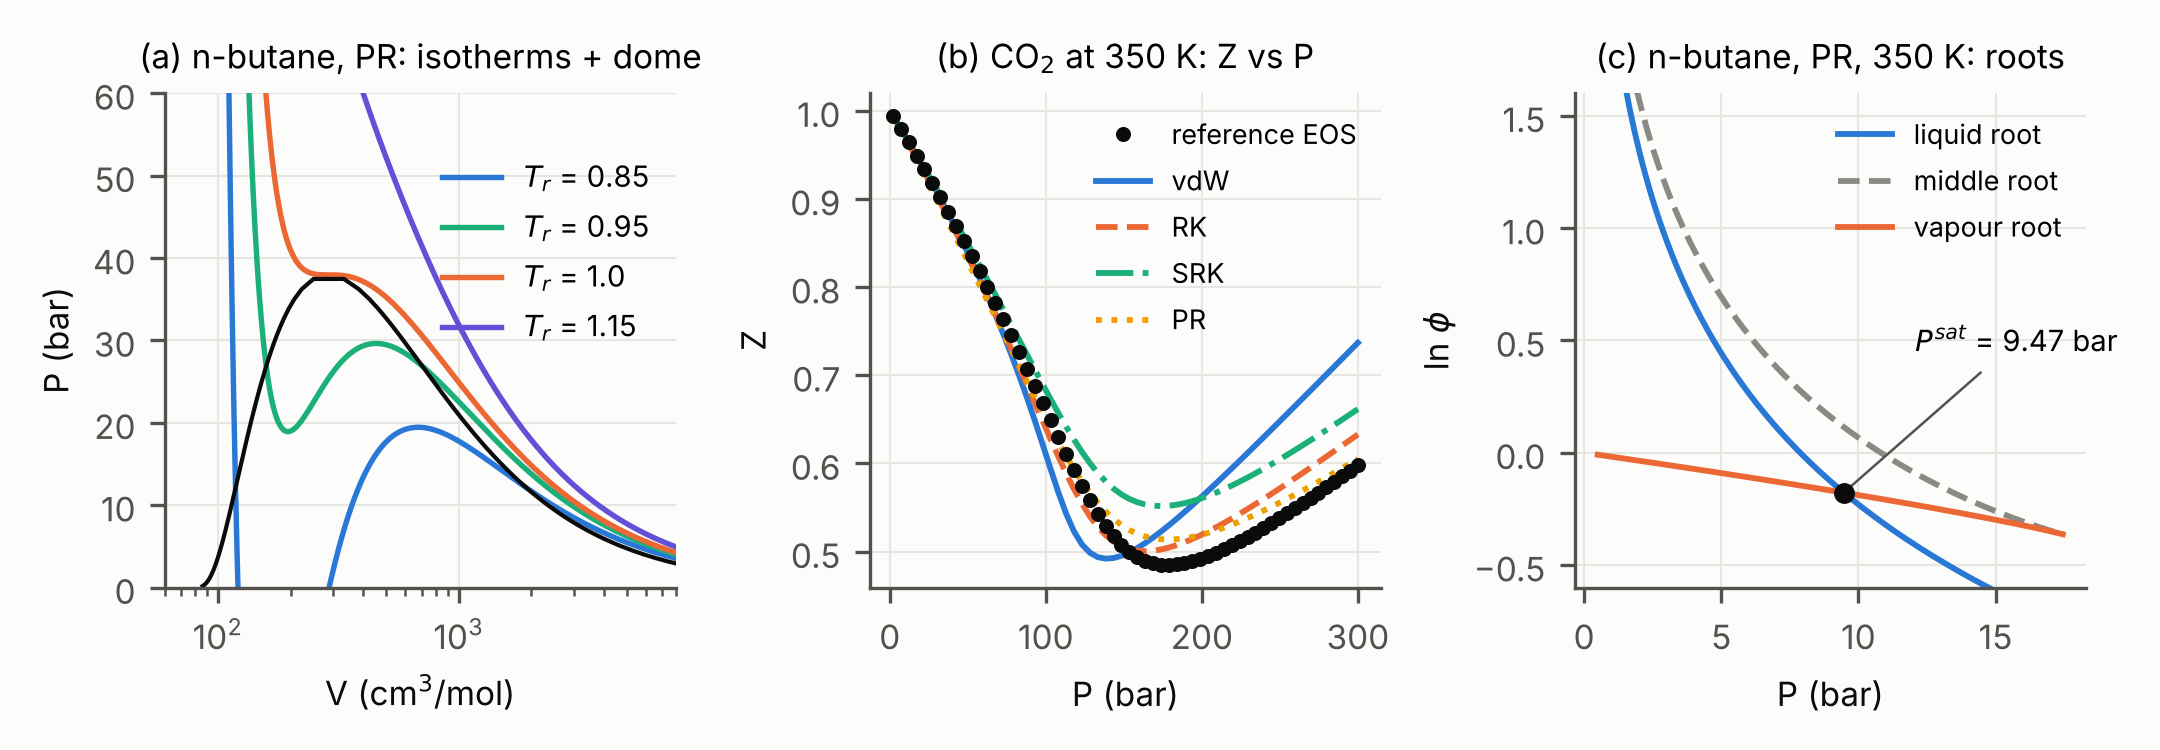
\includegraphics[width=\textwidth]{figures/fig1.png}
\caption{(a) PR isotherms and saturation dome of n-butane. (b) $Z$ of CO$_2$ at 350 K, four EOS vs.\ reference EOS. (c) $\ln\phi$ of the three roots of the cubic for n-butane (PR, 350 K): the stable root is the lower branch, and the liquid and vapour branches cross at $P^{sat}$ (equal fugacity).}\label{fig:1}
\end{figure}

\textbf{Fugacity.} Fig.~\ref{fig:1}c illustrates the stability rule: between the two spinodal pressures all three roots exist and the stable one is the lowest in $\ln\phi$; at $P^{sat}=9.47$ bar (experimental/reference 9.44 bar) the curves cross, $f^{sat}=7.93$ bar, $\phi^{sat}=0.837$. Fig.~\ref{fig:2}a gives $\phi$ of CO$_2$ at 350 K, which falls to 0.44 at 300 bar, i.e.\ the real gas has a much lower escaping tendency than an ideal gas at the same $P$.

\begin{figure}[h]\centering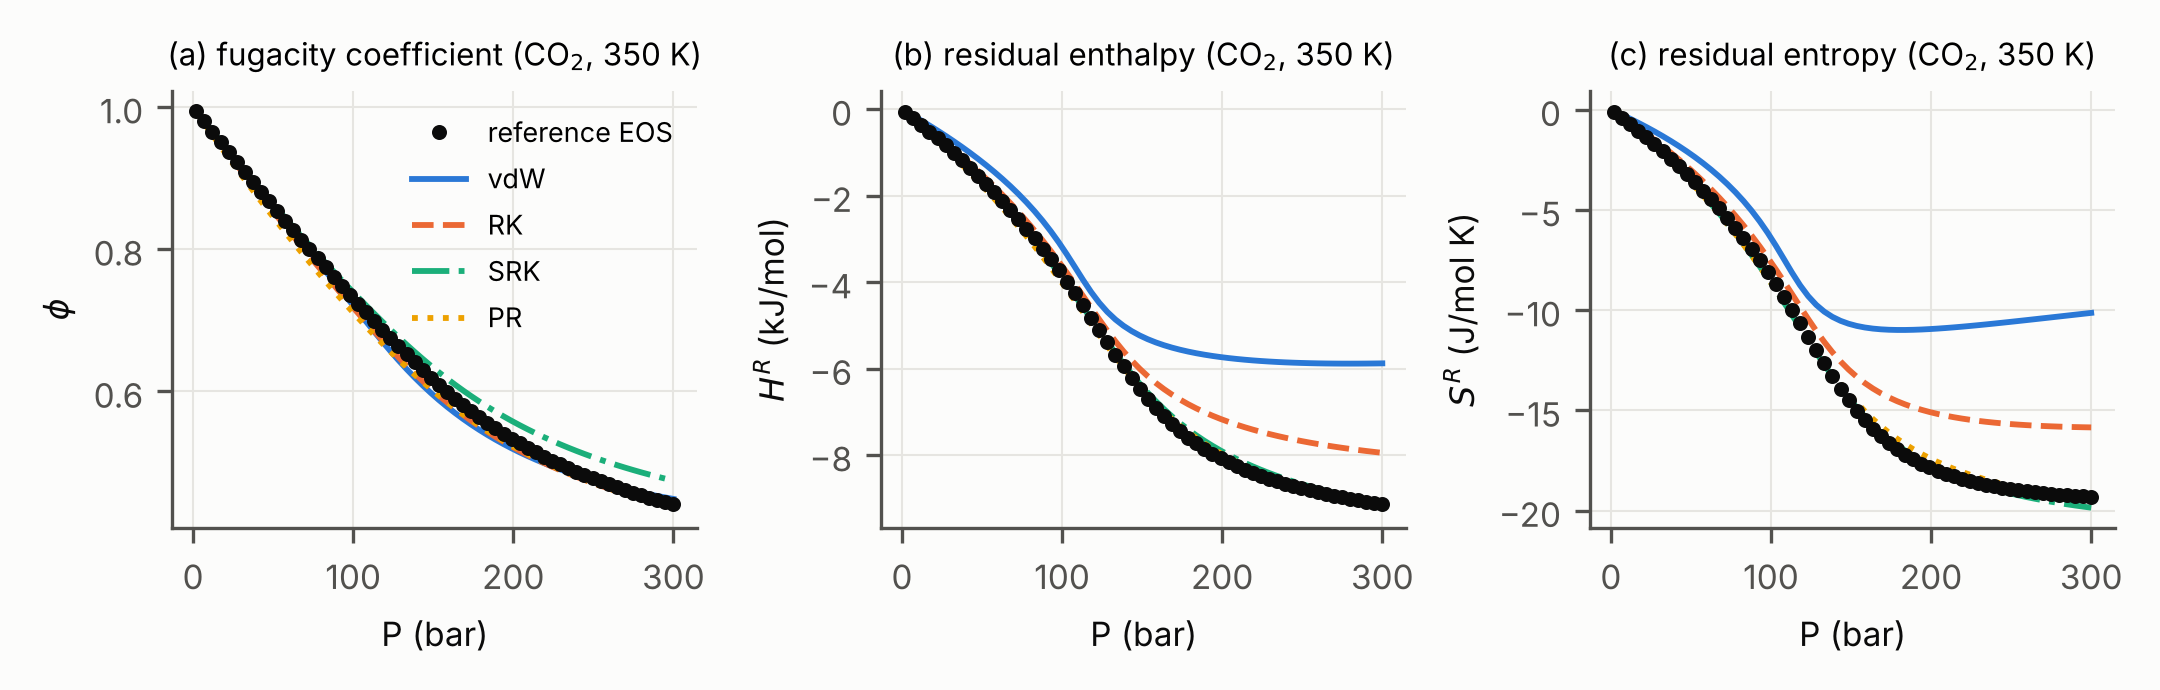
\includegraphics[width=0.92\textwidth]{figures/fig2.png}
\caption{Fugacity coefficient, residual enthalpy and residual entropy of CO$_2$ at 350 K versus pressure, four EOS and reference EOS.}\label{fig:2}
\end{figure}

\textbf{Enthalpy and entropy.} Fig.~\ref{fig:2}b,c show that attractive forces make $H^R$ and $S^R$ increasingly negative with $P$; vdW and RK underestimate the magnitude at high $P$ whereas SRK and PR follow the reference closely. Table~\ref{tab:ex} lists a worked state; Table~\ref{tab:acc} summarises the accuracy over a $T_r=1.1$--2, $P_r=0.2$--4 grid (20 states per gas, five gases: CO$_2$, CH$_4$, C$_3$H$_8$, N$_2$, NH$_3$) against the reference EOS.

\begin{table}[H]\centering\small
\begin{tabular}{lccccc}\toprule
CO$_2$, 350 K, 100 bar & $Z$ & $\phi$ & $f$ (bar) & $H^R$ (J/mol) & $S^R$ (J/mol K)\\\midrule
vdW & 0.6106 & 0.721 & 72.1 & $-3190$ & $-6.40$\\
RK & 0.6400 & 0.718 & 71.8 & $-3628$ & $-7.61$\\
SRK & 0.6831 & 0.740 & 74.0 & $-3900$ & $-8.64$\\
PR & 0.6511 & 0.711 & 71.1 & $-4014$ & $-8.63$\\
Reference EOS & 0.6610 & 0.731 & 73.1 & $-3830$ & $-8.34$\\\bottomrule
\end{tabular}\caption{Worked example (stable phase: supercritical-temperature gas).}\label{tab:ex}
\end{table}

\begin{table}[H]\centering\small
\begin{tabular}{lcccc}\toprule
Mean absolute error vs.\ reference (\%) & vdW & RK & SRK & PR\\\midrule
$Z$ & 5.2 & 2.1 & 3.3 & 2.0\\
$H^R$ & 14.9 & 4.7 & 3.6 & 9.2\\
$S^R$ & 21.1 & 7.0 & 5.7 & 8.0\\\bottomrule
\end{tabular}\caption{Average accuracy of the four EOS (100 states).}\label{tab:acc}
\end{table}

\textbf{Saturation and $\Delta H^{vap}$.} For n-butane at 350 K the program gives $P^{sat}$ = 16.60 (vdW), 11.41 (RK), 9.59 (SRK), 9.47 (PR) bar against 9.44 bar from the reference, and $\Delta H^{vap}$ = 8.17, 14.69, 17.55, 17.47 kJ/mol against 17.30 kJ/mol. Only SRK and PR, whose $\alpha(T_r)$ is fitted to vapour pressure through $\omega$, are accurate; the same holds for propane, CO$_2$ and NH$_3$ (e.g.\ NH$_3$ at 324.6 K: PR 20.97 bar, reference 21.08 bar). \textbf{Property change:} compressing N$_2$ from 300 K, 1 bar to 400 K, 100 bar (PR) gives $\Delta H=2633$ J/mol and $\Delta S=-30.77$ J/(mol K), versus 2927 J/mol and $-29.87$ J/(mol K) for an ideal gas, so neglecting the residual terms would be a 10\% error in $\Delta H$.

\section{Discussion and conclusions}
\begin{itemize}
\item The unified $(\sigma,\epsilon,\Omega,\Psi,\alpha)$ formulation lets one set of formulae (Eqs.~2--5) serve all four EOS; adding a further cubic EOS needs only one new row and its $\alpha(T_r)$ derivative.
\item Thermodynamic consistency is demonstrated numerically: $H^R,S^R$ obey the exact relations with $\ln\phi$, fugacities are equal at $P^{sat}$ and $\Delta H^{vap}$ satisfies Clapeyron's equation.
\item Accuracy: PR gives the best $Z$ and $P^{sat}$ overall, SRK the best $H^R,S^R$ in this gas set; vdW is only qualitative. Liquid volumes and the near-critical region are only approximate (PR gives $V^L$ 2\% low for n-butane at 350 K; no volume translation was used), and for strongly polar fluids (NH$_3$, water) errors are larger. In water, PR predicts a vapour pressure of 0.96 bar at 100$^\circ$C instead of 1.013 bar.
\item Limitations: pure components only; ideal-gas $C_p$ polynomials are valid for 298--1500 K; temperatures far below $T_r\approx0.45$ (extremely small $P^{sat}$) are not guaranteed.
\end{itemize}

\textbf{Files submitted:} \texttt{cubic\_eos.py} (program), \texttt{validate.py} (tests), \texttt{make\_figures.py} (figures and example data), this report. \textbf{Data/references:} Smith, Van Ness \& Abbott, \emph{Introduction to Chemical Engineering Thermodynamics}, Tables B.1 and C.1 and Ch.~3, 6, 10; Peng \& Robinson, Ind.\ Eng.\ Chem.\ Fundam.\ 15 (1976) 59; Soave, Chem.\ Eng.\ Sci.\ 27 (1972) 1197; Bell et al., CoolProp, Ind.\ Eng.\ Chem.\ Res.\ 53 (2014) 2498 (reference values used for comparison only).
\end{document}
